\chapter{Background on Probability and Statistics}
This chapter will discuss some statistical concepts that will be used to understand and build up the ideas behind the methodology of this paper, which is presented in the next chapter. With that said, the discussions are organized as follows: Section \ref{sec:descriptive_stat_method} will present the concept of Descriptive Statistics; Section \ref{sec:probability_method} will discuss the Probability Theory; and, Section \ref{sec:stat_graphs_method} will discuss the Statistical graphs or plots.

Further, the topics discussed here may be self-explanatory for Statisticians, ML researchers or those with Mathematical background. However, for the benefit of readers coming from humanities background, the paper will present the methodology as follows: mathematical formulas are formalized for purpose of brevity through Definition, Proposition, and Corollary, but immediate to these are explanations or examples aimed to be simple enough for non-statistician readers. As a guide, statisticians or ML researchers can simply read the Definition, Proposition, and/or Corollary. Whereas for humanities readers, the reading shouldn't not stress too much on the said mathematical formalities, and instead proceed to the discussions or examples immediate to it to aid with the understanding.
\section{Descriptive Statistics}\label{sec:descriptive_stat_method}
Among the basic statistical methodologies for summarizing information or data is what is known as Descriptive Statistics. From the name itself, these statistics are meant to convey simple descriptions of the data. For example, \textit{mean} and \textit{variance} are common statistics used for describing the data. The formulas for these statistics are given in the following definitions:
\begin{defnx}[Mean]\label{defn:mean}
Let $x_i, i\in\{1,\cdots,n\}$ where $n\in\mathbb{N}$, then the \textit{mean} of $x_i$s is defined as follows:
\begin{equation}
    \bar{x} = \sum_{i=1}^n x_i, \qquad\text{where}\;x_i \in\mathbb{R}.
\end{equation}
\end{defnx}
\begin{defnx}[Variance]
    Let $x_i, i\in\{1,\cdots,n\}$ where $n\in\mathbb{N}$ and let $\bar{x}$ be the mean defined in Defn. \ref{defn:mean} then the \textit{variance} of $x_i$s is defined as follows:
    \begin{equation}
        \mathbb{V}\text{ar}(x) = \frac{1}{n-1}\sum_{i=1}^n (x_i-\bar{x})^2, \qquad\text{where}\;x_i \in\mathbb{R}.
    \end{equation}    
\end{defnx}
\begin{defnx}[Standard Deviation]
Let $\sigma^2$ be the variance, then the standard deviation, denoted by $\sigma$, is defined as $\sigma:=\sqrt{\sigma^2}$, that is, square root of the variance.    
\end{defnx}
The mean is simply the average of the data points, while the variance is a single number that measures or summarizes the distances of the data points from the mean. The variance therefore measures how spread or varied the data points are. In practice, however, standard deviation is more popular for measure of variability since it doesn't get big easily due to the square root operator. Standard deviation is also the preferred metric for this paper.
\section{Probability Theory}\label{sec:probability_method}
Statistics is built around the concept of Probability Theory. Hence, it is important to understand how this mathematical theory behind the statistical concepts work. Probability theory is a discipline in itself. It is a branch of mathematics that aims at studying realizations or observations from random phenomena. It does this by using algorithms and models (\textit{see} discussion in Chapter \ref{ch:introduction} for understanding the model). These probability models are mathematical formula design to characterize or describe the patterns of data points. The simplest form of these models is the univariate probability density functions. However, before discussing these models, the idea behind it should be build up from ground up so that humanities readers can appreciate it. To do this, the discussion will proceed with the concept of probability.
\begin{defnx}[Probability]\label{defn:probability}
A probability is a mathematical concept that measures the likelihood or chance of some event to happen.
\end{defnx}
Indeed, this idea of probability is well known or is easily understood by many. So that, the probability that someone will die is 1, meaning 100\%, since that's how natures and biology work. Further, the probability of selecting one \arb[trans]{'ayAt} \arb{'ayAt} from \arb[trans]{sUraT 'l-fAti.hati} \arb{sUraT 'l-fAti.hati} through a random draw is one out of seven, assuming each \arb[trans]{'ayAt} \arb{'ayAt} has equal chances of being drawn.

Now, to gradually formalize the concept into mathematics, the succeeding definitions will be discussed to build up the definition of a probability distribution.
\begin{defnx}[Sample Space]
Let $\omega_1,\cdots,\omega_n, \forall n\in\mathbb{N}$ be the list of all possible outcomes of a random event or a phenomena, then the sample space, denoted by $\Omega$, is defined as the collection of all these possible outcomes including the empty set denoted by $\emptyset$.\qed
\end{defnx}
\begin{exmpx}\label{ex:sample_space}
Consider the random phenomenon or event where someone randomly picks a verse from the Qur'\=an, what is the probability that it will be a Meccan \arb{makkiyyaT} or a Medinan \arb{madaniyyaT} verse?

The possible output for such random event is either Meccan or Medinan. Suppose, we let Meccan to be denoted by $\omega_1$ and Medinan to be denoted $\omega_2$, then the sample space, which is the collection of all possible output is denoted as follows:
\begin{equation}\label{ex_eq:sample_space}
    \Omega:=\{\text{\arb{makkiyyaT}},\text{\arb{madaniyyaT}}\}=\{\text{Meccan}, \text{Medinan}\}=\{\omega_1,\omega_2\}
\end{equation}
It should be understood that $\emptyset$ is also included in $\Omega$, but is not written for brevity.
\qed
\end{exmpx}
\begin{defnx}[Event]
Let $\Omega=\{\omega_1,\cdots,\omega_n\}, \forall n\in\mathbb{N}$, be the sample space, then an event, denoted here as $\mathscr{A}$, is defined as the subset of the sample space, i.e., $\mathscr{A}\subseteq{\Omega}$.\qed
\end{defnx}
\begin{exmpx}
From Ex. \ref{ex:sample_space}, consider drawing two samples from the Qur'an, what is the sample space and give an example of a possible event?\\
\textit{Solution:} The sample space is given below:
\begin{align}
    \Omega=&\{(\text{\arb{makkiyyaT}},\text{\arb{makkiyyaT}}),(\text{\arb{makkiyyaT}},\text{\arb{madaniyyaT}}), (\text{\arb{madaniyyaT}}, \text{\arb{makkiyyaT}}), (\text{\arb{madaniyyaT}}, \text{\arb{madaniyyaT}})\}\nonumber\\
    =&\{(\text{Meccan},\text{Meccan}),(\text{Meccan},\text{Medinan}), \\
    &\;\;(\text{Medinan},\text{Meccan}), (\text{Medinan},\text{Medinan})\}\\
    =&\{(\omega_1,\omega_1),(\omega_1,\omega_2),(\omega_2,\omega_1),(\omega_2,\omega_2)\}
\end{align}
So that, if $\mathscr{A}$ is the event of drawing two \arb[trans]{'ayAt} \arb{'ayAt} from the Qur'\=an, then a possible event is given by 
\begin{equation}
    \mathscr{A}:=\{\text{\arb{madaniyyaT}}, \text{\arb{makkiyyaT}}\}=\{\text{Medinan}, \text{Meccan}\}=\{\omega_2,\omega_1\}
\end{equation}
Therefore, $\mathscr{A}\subseteq\Omega$, read as $\mathscr{A}$ is a subset of $\Omega$.\qed
\end{exmpx}
Now, going back to the discussion on the concept of probability above and reflect on the example given, that the probability that someone will die is 1; and that the probability of selecting one \arb[trans]{'ayAt} \arb{'ayAt} from \arb[trans]{sUraT 'l-fAti.hati} \arb{sUraT 'l-fAti.hati} through a random draw is one out of seven. It therefore begs the following questions: how does one solve this? Like how does it translate into a formal mathematical computation?

Indeed, to appreciate the motivation of the succeeding definitions, it is important to devise a logical approach to computing probability mathematically, and this should explain why the following definitions are defined the way they are.

Probability as already defined in Defn. \ref{defn:probability} is a measure, which will be formalized in Defn. \ref{defn:probability_measure}. Indeed, this is analogues to measuring an object's size using a tape measure. So, when someone attempts to measure an object's size, there are conditions for the space of the object to be measurable. The first expectation is that, the space or area can be measured in several ways. Either measuring it as a whole, or measuring it piece by piece from its partitions. Now, measuring it as a whole using tape measure should be straightforward. However, measuring it by pieces can have several cases, and all of these should end up to the same measuring. These cases accounts for the fact that when dealing with pieces of the surface one can start with different sizes of the pieces to be measured. So that, all the collections of all these possible configurations of pieces are mathematically called $\sigma$-algebra, and this collection should include the following:
\begin{enumerate}
    \item The 0 size piece, that is, the object's measurement should start at 0;
    \item The remainings of the pieces given the pieces already measured;
    \item The union of all the pieces.
\end{enumerate}
The above explanation for the $\sigma$-algebra is condensed in to the following mathematical definition:
\begin{defnx}[$\sigma$-algebra]\label{defn:sigma_algebra}
Let $\Omega:=\{\omega_1,\cdots,\omega_n\}, \forall n\in\mathbb{N}$, then the collections of all disjoint partitions, which are the events, are defined as the $\sigma$-algebra or $\sigma$-field, denoted here as $\mathfrak{F}$, and should satisfy the following conditions:
\begin{enumerate}
    \item The empty set $\emptyset\in\mathfrak{F}$
    \item If $\mathscr{A}\in\mathfrak{F}$, then the complement $\Omega\backslash\mathscr{A}$ is also an element of $\mathfrak{F}$
    \item If $\mathscr{A}_1,\mathscr{A}_2,\cdots$ is a countable sequence of sets in \mathscr{A}, then the $\bigcup_{i=1}^{\infty}\mathscr{A}_i$ is also an element of $\mathfrak{F}$
\end{enumerate}\qed
\end{defnx}
\begin{exmpx}
Given the sample space $\Omega:=\{\text{Meccan},\text{Medinan}\}$, the $\sigma$-algebra is
\begin{align}
    \mathfrak{F}=&\{\text{Meccan},\text{Medinan},(\text{Meccan},\text{Medinan}),\nonumber\\
    &\;\;(\text{Meccan},\text{Meccan}), (\text{Medinan},\text{Meccan}),\nonumber\\
    &\;\;(\text{Medinan},\text{Medinan}),\emptyset\}
\end{align}
\qed
\end{exmpx}
\begin{defnx}[Probability Measure]\label{defn:probability_measure}
Let $\Omega$ be the \textit{sample space}, $\mathfrak{F}$ be the $\sigma$-algebra, $\mathbb{P}$ be the probability measure, then the probability of a set $\mathscr{A}, \mathscr{A}\in\mathfrak{F}$, on the probability space $(\Omega,\mathfrak{F},\mathbb{P})$, denoted by $\mathbb{P}(\mathscr{A})$, satisfies the following properties:
\begin{enumerate}
    \item Non-negativity: For any set $\mathscr{A}, \mathbb{P}(\mathscr{A})\geq 0$
    \item Normalization: $\mathbb{P}(\Omega)=1$
    \item Countable additivity: For any sequence of disjoint sets $\mathscr{A}_1,\mathscr{A}_2,\cdots$ in $\mathfrak{F}$, such that the union $\bigcup_{\forall i \in\mathbb{N}}\mathscr{A}_i$ is also in $\mathfrak{F}$, we have: $\mathbb{P}\left(\displaystyle\bigcup_{\forall i\in\mathbb{N}}\mathscr{A}_i\right)=\displaystyle\sum_{\forall \in\mathbb{N}}\mathbb{P}(\mathscr{A}_i)$
\end{enumerate}
\qed
\end{defnx}

Basically, the idea of Defn. \ref{defn:probability_measure} is to define the concept of "measure" in general sense, although above is a special measure called probability measure. As before, one can think of this probability measure like a tape measure in simple sense. This tape measure has some properties that should be expected for a measurement tool. The first property or condition is that the probability measure has to be positive. Indeed, if we use any tape measure for measuring length, never will someone get a negative measure like -2cm length. It always has to be positive. Further, the second condition to expect is that for this type of tape measure called probability measure, the total measure of all objects available in the given space should be equal to 1. That is, the total is normalized to 1. Think of this like 100\% coverage if we measure all of the objects. Lastly, for any object, this tape measure should be able to measure the object through partitions, such that the measure of the union of these partitions is equal to the sum of the measure of each partition. All of these conditions are logical criteria for a general idea of "measure," although the normalization part above is unique for probability measure. Note that, the concept of proability measure here should not be confined to measuring length as in the analogy, it should generalize to measuring volume and complex objects in general.
\begin{defnx}[Random Variable]
Let $\Omega$ be the sample space, and $\mathbb{R}$ be the set of all real numbers, then a random variable $X$ is a function defined as $X:\Omega\rightarrow\mathbb{R}$.\qed
\end{defnx}
\begin{exmpx}\label{ex:ayah_prob}
Consider the example of drawing a random verse or \arb[trans]{'ayAt} \arb{'ayAt} again, what is the probability that it will be an \arb[trans]{'ayAt} \arb{'ayAt} from \textit{s\=urah l-baqara}'s \arb[trans]{'ayAt} \arb{A"'yaTu sUraT 'l-baqaraT} or the Chapter of Cow?

The answer to this is 4.59\% probability, this is because there are 286 \arb[trans]{'ayAt} \arb{'ayAt} and there are 6236 verses in the Qur'\=an, so that the probability is $\frac{286}{6236}=0.04586$. The assumption here is that all of the \arb[trans]{'ayAt} \arb{'ayAt} in the Qur'\=an have equal chances of being picked up or drawn.
\qed
\end{exmpx}
\begin{exmpx}\label{ex:binom_manual}
To apply the concept so far, consider again Ex. \ref{ex:ayah_prob}, what is the probability of getting 5 \textit{s\=urah l-baqara}'s \arb[trans]{'ayAt} \arb{A"'yaTu sUraT 'l-baqaraT} if we randomly pick 20 \arb[trans]{'ayAt} \arb{'ayAt} in total from the Qur'\=an?\\
\textit{Solution.} The following are given:
\begin{itemize}
    \item $n=20$ independent trials of drawing $x=5$ \arb{'ayAt} from the Qur'\=an
    \item Each trial has two possible outcomes: \arb[trans]{na`am} \arb{na`am} meaning Yes or \arb[trans]{lA} \arb{lA} meaning No. That is, if the \arb[trans]{'ayAt} \arb{'ayAt}  is from the \textit{s\=urah l-baqara} \arb{sUraT 'l-baqaraT} then its \arb{na`am}, otherwise \arb{lA}.
\end{itemize}
Now, the sample space consists of all possible sequences of 20 \arb{na`am} and \arb{lA}. That is,
\begin{align}
    \Omega=\{&
        (\text{\arb{lA}},\text{\arb{na`am}},\text{\arb{lA}},\cdots,\text{\arb{na`am}}),\\
        &(\text{\arb{lA}},\text{\arb{na`am}},\text{\arb{lA}},\cdots,\text{\arb{lA}}),\\
        &\qquad\qquad\vdots\\
        &(\text{\arb{lA}},\text{\arb{lA}},\text{\arb{lA}},\cdots,\text{\arb{lA}})\}.
\end{align}
In total, there are $20^2=400$ possible samples in the sample space $\Omega$. Further, from Ex. \ref{ex:ayah_prob}, the probability of getting a \textit{s\=urah l-baqara}'s \arb[trans]{'ayAt} \arb{A"'yaTu sUraT 'l-baqaraT} is 0.0459 or 4.59\%. Therefore, if $X$ is the random variable of an event of drawing an \arb[trans]{'ayAt} from the Qur'\=an, if we assign \arb{lA}  and \arb{na`am} as either 0 or 1, respectively, then this would imply that mathematically $\mathbb{P}(X=1)=0.0459$. In addition, the probability of getting an \arb[trans]{'ayAt} \arb{'ayAt} from other \textit{s\=urah} \arb{sUraT} would be

\begin{equation}    
\mathbb{P}(X=0)=1-\mathbb{P}(X=1)=1-0.0459=0.9541.
\end{equation}

Further, let $Z$ be the random variable for the event of getting $n$ \arb{na`am} from 20 trials, then the problem is now equivalent to finding the number of ways to choose $n$ possible positions out of 20 in the collection or set. This can be solved using the \textit{combination} formula as shown below:
\begin{align}
    n \choose x &= \frac{n!}{r!(n-r)!}\Rightarrow{20 \choose 5} = \frac{20!}{5!(20-5)!}=15,504. 
\end{align}
That is, there are 15,504 possible cases of 5 positions' configuration for \arb{na`am} in a 20 trial. Moreover, in each of these samples 5 has a probability of $\mathbb{P}(X=1)=0.0459$, while the remaining 15 has a probability of $\mathbb{P}(X=0)=0.9541$. So that,
\begin{align}
    \mathbb{P}(Z=5)&=184,756\times\mathbb{P}(X=1)^{5}\times\mathbb{P}(X=0)^{20-5}\nonumber\\
    &=15,504\times0.0459^{5}\times0.9541^{20-5}\nonumber\\
    &=0.0016.
\end{align}
Hence, there is a 0.16\% probability of getting 5 \textit{s\=urah l-baqara}'s \arb[trans]{'ayAt} \arb{A"'yaTu sUraT 'l-baqaraT} when randomly drawing 20 \arb{'ayAt} from the Qur'\=an.
\qed
\end{exmpx}
Note that Ex. \ref{ex:binom_manual} can be solved using a known formula in probability called \textit{Binomial} mass function, which is a model that can be used to describe the event of getting 5 \textit{s\=urah l-baqara}'s \arb[trans]{'ayAt} \arb{A"'yaTu sUraT 'l-baqaraT} on a 20 random samples of Qur'\=an's \arb{'ayAt}. The {Binomial} mass function is specifically a probability mass/density function model. The following section will discuss the Statistical Graphs, which will cover the concept of frequency distribution, the one modeled or characterized by the probability mass/density function.
\section{Statistical Graphs}\label{sec:stat_graphs_method}
Graphs or plots are data visualization tools that are useful for exploratory data analysis apart from the Descriptive Statistics discussed above. It supplements the Descriptive Statistics findings through shapes visualized in the graphs. Among the popular statistical graphs is the bar graph. An example of this is given in Figure \ref{fig:ayah_word_count}. Other graphs used are the box plots and the density plots which is also in Figure \ref{fig:ayah_word_count}
\subsection{Box, Density, and Histogram Plots}
While most statistical plots are easy to understand like bar graphs and scatter plots, others like Box, Density, and Histogram plots may not be easy to comprehend for someone with no Statistical background. This section will discuss how it is interpreted. Let's use Figure \ref{fig:ayah_word_count}, Figure \ref{fig:ayah_word_count_with_desc} for easy reference in this section.
\begin{figure}[!b]
    \centering
    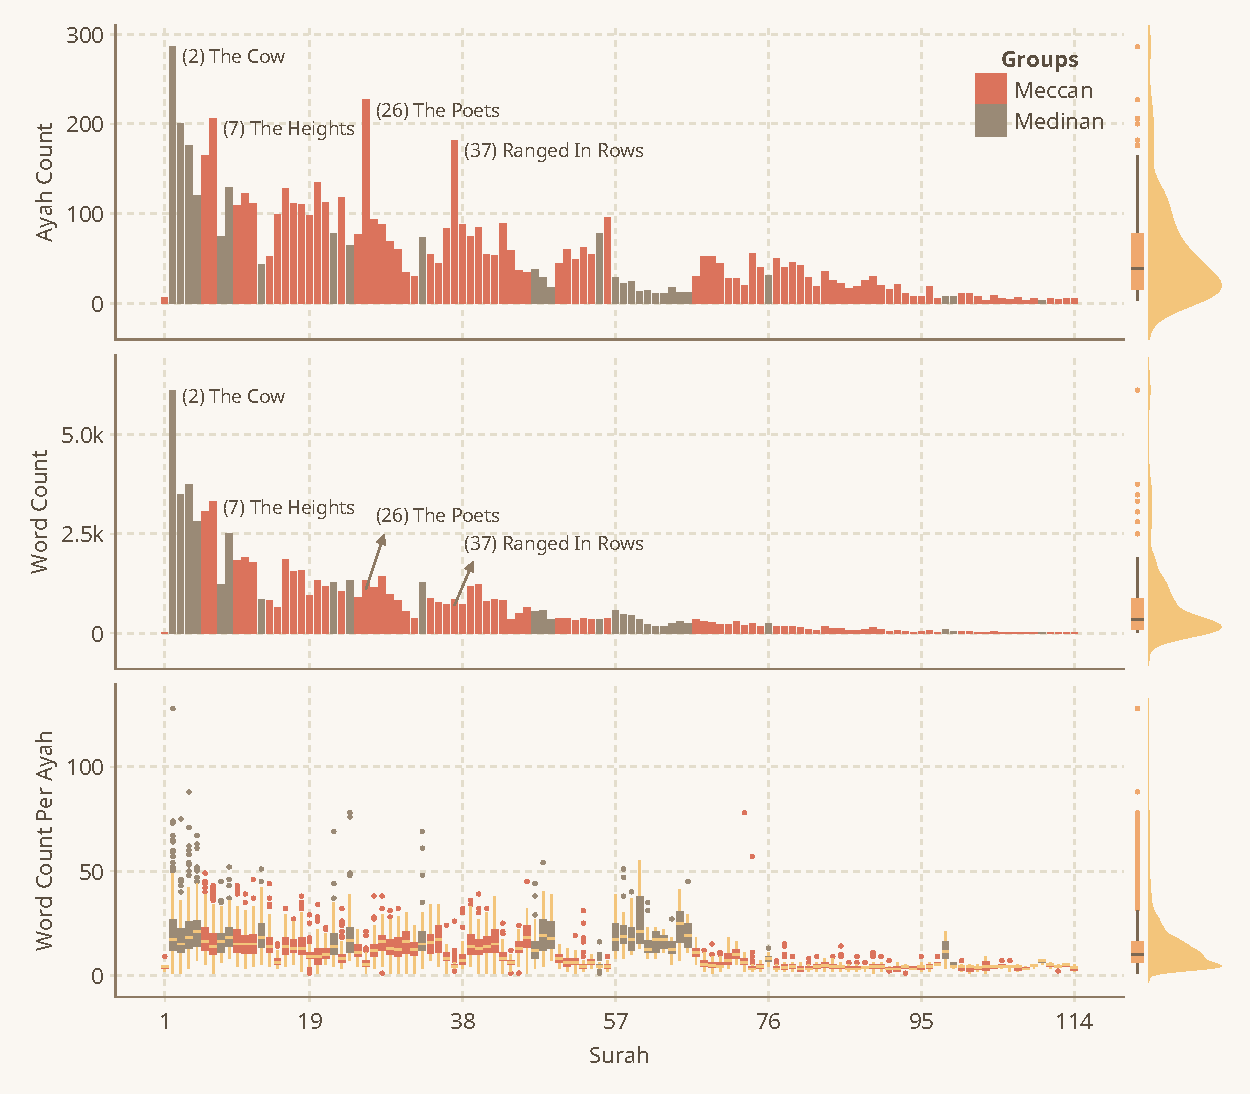
\includegraphics[width=\textwidth]{img/plot1.pdf}
    \caption{Statistics of the words and \arb[trans]{ayAt} \arb{ayAt} (verses) of the Qur'\=an}
    \label{fig:ayah_word_count_with_desc}
\end{figure}

As shown in Figure \ref{fig:ayah_word_count_with_desc}, both the Box and Density plots are tied to each other. This is indeed the case because both are describing the same information but presented in different style of visualization. In fact, Histogram is also used to describe the same information as the Box and Density, and the three are therefore related. So much so, that the three can be put into one graph. As to how to interpret these, readers are referred to for further details \textcolor{red}{[to add reference]}.
\begin{exmpx}[Frequency Distribution]\label{ex:frequency_distribution}
Consider again the task of drawing an \arb[trans]{'ayAt} \arb{'ayAt} from the Qur'\=an, suppose the \arb[trans]{'ayAt} \arb{'ayAt} are separated into \arb{makkiyyaT} Meccan and \arb{madaniyyaT} Medinan, what is the probability of getting at most 10 \arb[trans]{kalimAt} \arb{kalimAt} or words in a sampled \arb[trans]{'ayAt} \arb{'ayAt} from \arb{makkiyyaT} Meccan \textit{surah}s \arb{sUr}?\\
\textit{Solution:} To answer this, Figure \ref{fig:meccan_medinan_word_count_per_ayah} shows the \textit{histograms} with the \textit{box plots} and the \textit{rainclouds} plots. The figure shows the frequency of the \arb[trans]{kalimAt} \arb{kalimAt} or words in a sampled \arb[trans]{'ayAt} \arb{'ayAt}. This frequency describes the distribution of the \arb[trans]{kalimAt} \arb{kalimAt}. To interpret this, the Medinan \arb{madaniyyaT} histogram shows that most of the \arb[trans]{'ayAt} \arb{'ayAt} have about 10 to 20 \arb[trans]{kalimAt} \arb{kalimAt} or words in total. This conclusion is based on the where the box of the box plot is located, which also corresponds to the area where the bars of the histogram are high, and also where most of the points or 'droplets' from the rainclouds plot are congested. With that said, \textit{historgram}, \textit{box plot}, and \textit{rainclouds} are related and are telling the same story from different perspectives. It should be noted that, the rainclouds plot is not a common visualization tool. 

Now, comparing the numbers from Medinan \arb{madaniyyaT} to the \arb[trans]{'AyAt 'l-makkiyyaTu} \arb{'AyAt 'l-makkiyyaTu}, there are about 5 to 15 \arb[trans]{kalimAt} \arb{kalimAt} to expect per \arb[trans]{'ayAt} \arb{'ayAt} based on Figure \ref{fig:meccan_medinan_word_count_per_ayah}. 

\begin{figure}[!t]
    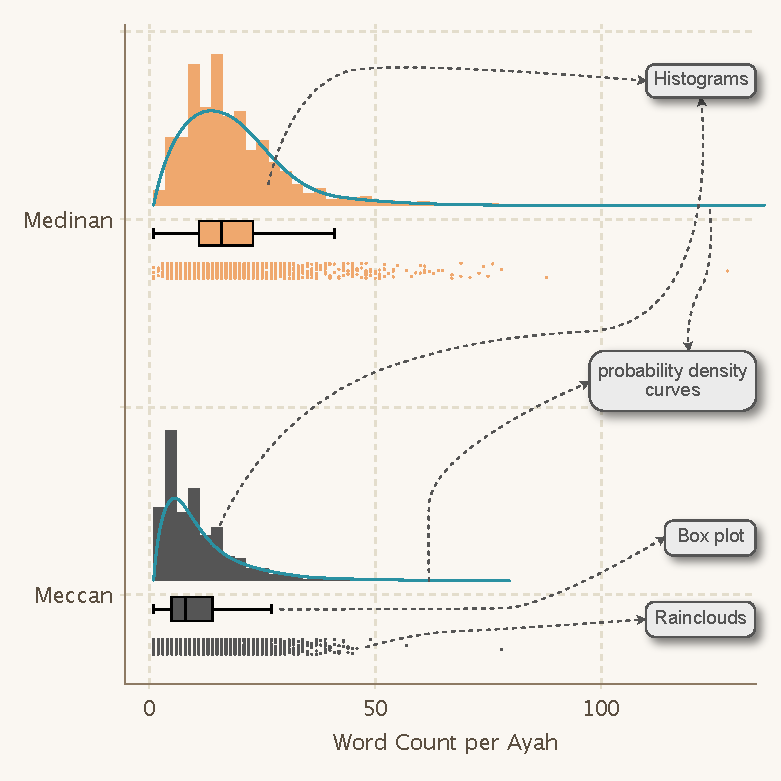
\includegraphics[width=\textwidth]{img/plot3.pdf}
    \caption{Probability density function plot of word count per \arb[trans]{'ayAt} \arb{'ayAt} by revelation location, in relation to its box plot and rainclouds.}
    \label{fig:meccan_medinan_word_count_per_ayah}
\end{figure}

The question has not been answered yet though, the above discussions only explains how to interpret the graphs in Figure \ref{fig:meccan_medinan_word_count_per_ayah}. So to answer the question, one simply needs to total the number of \arb[trans]{'AyAt} \arb{'AyAt} with at most 10 \arb[trans]{kalimAt} \arb{kalimAt} or words and divide this with the total number of \arb[trans]{'AyAt 'l-makkiyyaTu} \arb{'AyAt 'l-makkiyyaTu}. The answer is as follows, and this is part of the result of this paper: there are 4613 \arb[trans]{'AyAt 'l-makkiyyaTu} \arb{'AyAt 'l-makkiyyaTu}, and out of these is 2602 \arb[trans]{'AyAt 'l-makkiyyaTu} \arb{'AyAt 'l-makkiyyaTu} with at most 10 words. Therefore, the probability is $\frac{2602}{4613}=0.612$ or 61.2\% probability. Formally, if $X$ is the random variable of the event of observing at most 10 \arb[trans]{kalimAt} \arb{kalimAt} in a \arb[trans]{'AyAt 'l-makkiyyaTu} \arb{'AyAt 'l-makkiyyaTu}, then 
\begin{align}
    \mathbb{P}(X\leq 10)=&\sum_{x=0}^{10}\mathbb{P}(X=x)\label{ex_eq:prob_lesseq_10}\\
    =&\mathbb{P}(X=0)+\mathbb{P}(X=1)+\mathbb{P}(X=2)+\cdots+\mathbb{P}(X=10)\label{ex_eq:freq_dist_prob1..10}\\
    =&0+\frac{24}{4613}+\frac{172}{4613}+\cdots+\frac{222}{4613}\label{ex_eq:freq_dist_probval1..10}\\
    =&\frac{2602}{4613}=0.612\label{ex_eq:prob_0612}
\end{align}

From Eq. \ref{ex_eq:freq_dist_prob1..10}, $\mathbb{P}(X=0)$ is the probability of observing zero \arb[trans]{kalimaT} \arb{kalimaT} in a \arb[trans]{'AyAt 'l-makkiyyaTu} \arb{'AyAt 'l-makkiyyaTu}, and $\mathbb{P}(X=1)$ is the probability of observing one \arb[trans]{kalimaT} \arb{kalimaT} in a \arb[trans]{'AyAt 'l-makkiyyaTu} \arb{'AyAt 'l-makkiyyaTu}, and so on. The numbers in Eq. \ref{ex_eq:freq_dist_probval1..10} are the number of \arb[trans]{'AyAt 'l-makkiyyaTu} \arb{'AyAt 'l-makkiyyaTu} having zero, one, two, to ten \arb[trans]{kalimAt} \arb{kalimAt}.
\qed
\end{exmpx}
\section{Population and Sample}
Statistics is a branch of science that is concerned with understanding how the data behave based on a sample---a small set of the said data. It uses statistical methodologies to understand these behavior such as probability mass/density function, and use the findings from these tools on the sampled data as a conclusion for the population---the overall data.

Figure \ref{fig:pop_sample} illustrates the relation of population and sample data. A good example of this is the political surveys on the pulse of the nation on the candidates prior to election. Private entities like PulseAsia\footnote{\url{https://pulseasia.ph/}} and Social Weather Station\footnote{\url{https://www.sws.org.ph/swsmain/home/}} (SWS) do their survey by  sampling from the total population of the Philippines, hence the name survey.

The statistics computed from the surveys like the percentage of votes for particular political candidate are referred as estimates, this is because the computation was done in a sample of the population and not on the population itself. It is therefore important that for these estimates to be accurate representation of the nation's opinion, it has to be representative of the population. That is, the sample shouldn't be bias and leaning to the opinions of the few only and not of the whole nation.

The importance of the sample data as illustrated below follows from the fact that it saves time and cost since interviewing 2500 compared to 100,000 is better compromise for the estimated vote percentages. Further, since these samples requires to well represent the population, the computations of the statistics are estimated using statistical models, like probability mass/density functions, and other models like linear and nonlinears discussed in Section \ref{sec:stat_modeling}. The next example will illustrate the idea population and sample, and how probabilistic modeling can help in understanding insights and answering more questions.
\begin{figure}[t]
    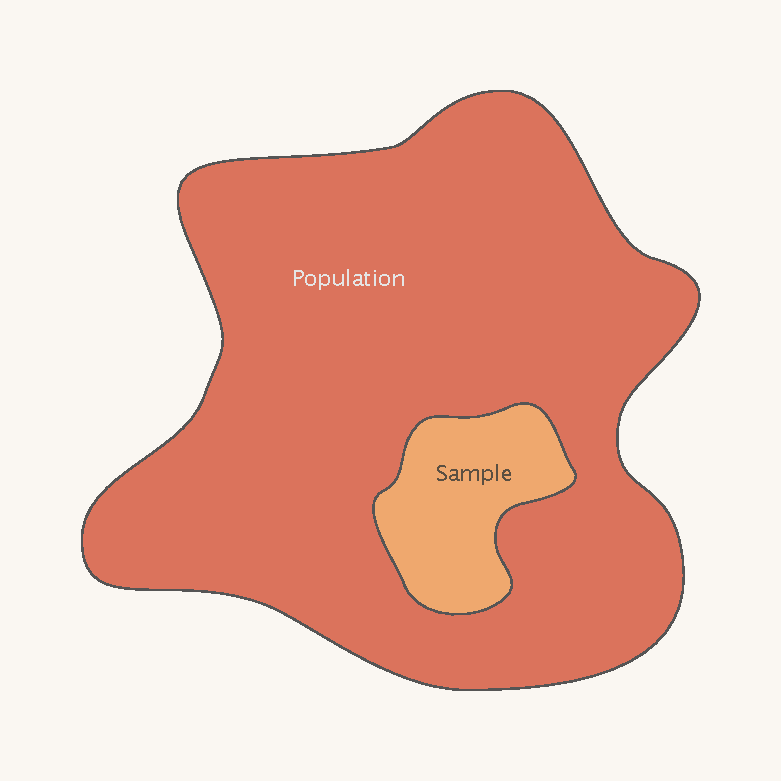
\includegraphics[width=\textwidth]{img/pop_sample.pdf}
    \caption{Population and sample illustration}
    \label{fig:pop_sample}
\end{figure}
\begin{exmpx}\label{ex:population_sample_distribution_meccan_words}
Consider the task of sampling 100 \arb[trans]{'AyAt} \arb{'AyAt} from the population of \arb[trans]{'AyAt 'l-makkiyyaT}, describe the statistics of the population and the sample.\\
\textit{Solution:} In Statistics, there are several ways to sample from data, the simplest approach is through the use of \textit{uniform distribution}, that is, the sampling assumes that all data from the population are distributed equally, in the sense that all data points have equal chance of being selected. The other approach is through a \textit{weighted distribution}, where a probability is assigned to each of the data points in the population, so that, the selection will be biased to those with high probability. Figure \ref{fig:meccan_words_sampling} shows the graphs or plots of the population distribution of \arb[trans]{kalimAtu 'l-makkiyyaT} \arb{kalimAtu 'l-makkiyyaT}, which is presented as the top plot, this distribution of \arb{kalimAtu 'l-makkiyyaT} is the same one shown in the bottom plot of Figure \ref{fig:meccan_medinan_word_count_per_ayah}. 

To draw 100 samples from the said population, a simple random sampling without replacement (SRSWOR) is used for selecting or drawing samples. SRSWOR works by randomly selecting sample from the population and then setting it aside as the first sample. The resulting 100 samples are plotted in the bottom plot of Figure \ref{fig:meccan_words_sampling}.

As discussed above, the sample needs to be representative of the population. Figure \ref{fig:meccan_words_sampling} shows that the sampling distribution has more or less the same shape as the population. So that, the statistics are shown in Table \ref{tbl:meccan_words_pop_sample_stats}. From the said table, it can be seen that in terms of centrality, the both data are almost the same, for example the mean is 12.42 for the population and 10.64 for the sample. The reason why the mean in the population is much higher is due to the outlier in the population, which is seen in the extent of the tail of the Kernel Density Estimate in Figure \ref{fig:meccan_words_sampling}. In fact, this is seen in the Median in Table \ref{tbl:meccan_words_pop_sample_stats}, where  the estimate are almost the same. This is because the median is not affected by the outlier. However, the variance did suffer from the outlier in the population, with 50\% reduction in the sample variance, 54.15 to 48.96. The sample will less likely get the outlier as the sample since the outlier is only one observation from the 4163 total Meccan surahs.

The estimates got from the sample ideally are taken from a probabilistic model fitted into the sample data. This computation will be discussed in the next example.

\begin{table}
    \caption{Descriptive statistics of the population and sample data of \arb[trans]{kalimAtu 'l-makkiyyaT} \arb{kalimAtu 'l-makkiyyaT}}
    \label{tbl:meccan_words_pop_sample_stats}
    \begin{tabularx}{\textwidth}[!h]{XXXXl}
        \toprule
        Data&Mean&Median&Variance&Std. Deviation\\
        \midrule
        Population&10.28&8&54.15&7.36\\
        Sample&10.64&9&48.96&7.00\\
        \bottomrule
    \end{tabularx}
\end{table}
\begin{figure}[t]
    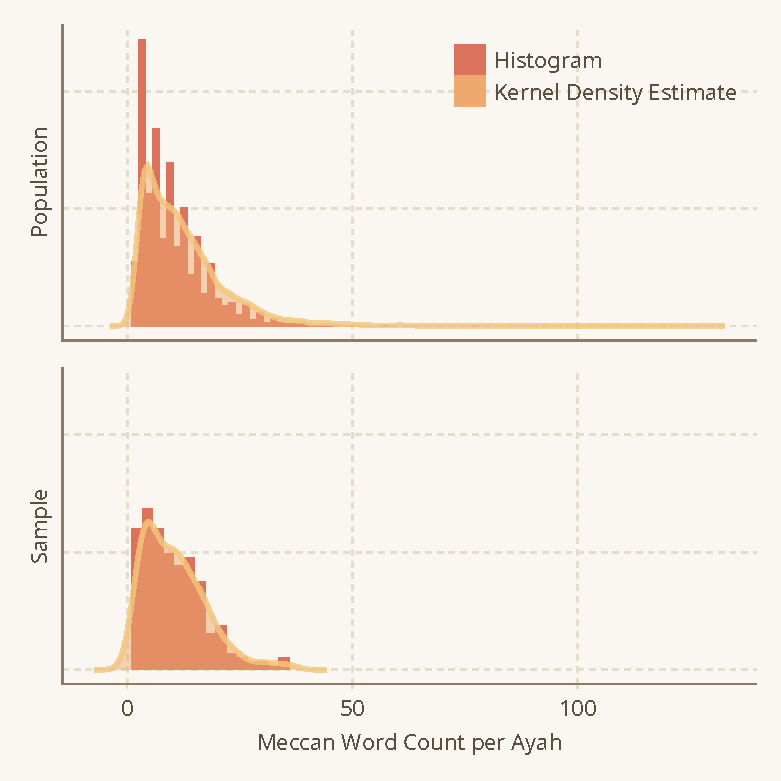
\includegraphics[width=\textwidth]{img/plot5.pdf}
    \caption{Population and sample distribution of Meccan }
    \label{fig:meccan_words_sampling}
\end{figure}
\qed
\end{exmpx}
\begin{exmpx}
Consider again Ex. \ref{ex:population_sample_distribution_meccan_words}, suppose the sample data is the only data available, how will you compute the probability of getting exactly 35 \arb[trans]{kalimAtu 'l-sUratu 'l-makkiyyaTu} \arb{kalimAtu 'l-sUratu 'l-makkiyyaTu}?\\
\textit{Solution:} To answer this question, one might approach this using the frequency distribution as in Ex. \ref{ex:frequency_distribution}. However, the use of frequency distribution from the said example is applicable since that deals with the population data, which is already the true probability, and there is no need to do some estimation. It is like try to get the average height of male Filipinos in the Philippines by doing census across the population, for such case, why would you do an estimate if you have all the census data of all heights of the Filipino, wouldn't it be easier to just do the average computation directly? This is the analogy for the frequency distribution used in Ex. \ref{ex:frequency_distribution}, that is, no need to do some estimation. However, for this problem, the assumption is that only the sample is available, that is, not all of the population is available. With that said, the best solution is to do some estimation. Now, doing an estimation is possible using the samples only, that is, using the idea of frequency distribution but this time applying it on the sample. This is becaus the sample was done using a random sampling, which more or less representative of the population. However, using this approach may possess a problem, let's see what that problem will likely be by forcing the approach in Ex. \ref{ex:frequency_distribution}, following the computation as in Eq. (\ref{ex_eq:prob_lesseq_10}) to Eq. (\ref{ex_eq:prob_0612}). 

Let $X$ again be the random variable of an event of observing 35 \arb[trans]{kalimAt} \arb{kalimAt}, this time from the sample, then
\begin{equation}\label{eq:probx_eq_35}
    \mathbb{P}(X=35)=\begin{cases}
        \displaystyle\frac{0}{250}=0,&\text{if sample data}\\
        \displaystyle\frac{5}{4613}=0.0011,&\text{if population data}
    \end{cases}
\end{equation}
From the Eq. \ref{eq:probx_eq_35}, it shows that if we use the sample data for estimating the probability of observing 35 \arb{kalimAt}, then the answer above is 0, meaning by estimate there is a 0 chance of observing a 35 \arb{kalimAt} from a \arb[trans]{'AyAtu 'l-makkiyyaTu} \arb{'l-sUrAtu 'l-makkiyyaTu}. This conclusion is indeed misleading, since according to the population data, there are \arb[trans]{'AyAtu 'l-makkiyyaTu} \arb{'AyAtu 'l-makkiyyaTu} that has 35 \arb[trans]{kalimAt} \arb{kalimAt}. 

So, how to properly estimate this then? This is where the concept of probabilistic modeling comes in. For this problem, the data is count, and that the event of observing 10 \arb[trans]{kalimAtu 'l-sUratu 'l-makkiyyaTu} \arb{kalimAtu 'l-sUratu 'l-makkiyyaTu} in an \arb{'AyaT} is known to be best modeled by a Poisson distribution defined in Defn. \ref{defn:poisson_mass_function}. Ex. will discuss how to solve this.   44 
\end{exmpx}
\section{Probability Distributions}
\begin{defnx}[Poisson Mass Function]\label{defn:poisson_mass_function}
Let $X$ be a random variable and let $\lambda>0$ be a parameter, then if $x$ is the random value, then the \textit{Poisson} mass function is given by:
\begin{equation}
    \mathbb{P}(X=x)=\frac{\lambda^x\exp(-\lambda)}{x!}
\end{equation}
\end{defnx}
\begin{defnx}[Normal Density Function]
Let $Y$ be a random variable and let $\mu\in\mathbb{R}$ and $\sigma\in\mathbb{R}$ be the mean and variance parameters, if $y$ is the random value, then the \textit{Gaussian} or \textit{Normal} density function is given below:
\begin{equation}
    \mathbb{P}(Y=y):=\frac{1}{\sqrt{2\pi\sigma^2}}\exp\left\{-\frac{(y-\mu)^2}{\sigma^2}\right\},\quad\text{where}\;-\infty<y<\infty
\end{equation}
\end{defnx}
\begin{defnx}[Dirichlet Density Function]
Let $\mathbf{Y}$ be a vector random variable with a random value $\mathbf{y}:=[y_1,\cdots,y_k]^{\text{T}}$ and let $\boldsymbol{\alpha}:=[\alpha_1,\cdots,\alpha_k]^{\text{T}}$ be the parameters, then the \textit{Dirichlet} density function is defined as
\begin{equation}
    \mathbb{P}(\mathbf{X}=\mathbf{x};\boldsymbol{\alpha}):=\frac{1}{B(\boldsymbol{\alpha})}\prod_{i=1}^kx_i^{\alpha_i-1},
\end{equation}
where,
\begin{equation}
    B(\boldsymbol{\alpha}):=\frac{\displaystyle\prod_{i=1}^k\Gamma(\alpha_i)}{\Gamma\left(\sum_{i=1}^k\alpha_i\right)}
\end{equation}
\qed
\end{defnx}
\begin{defnx}[Multinomial Mass Function]
Let $\mathbf{X}$ be a vector random variable with a random value $\mathbf{x}:=[x_1,\cdots,x_k]^{\text{T}}$ such that $x_i\geq 0,\forall i \in[1,k]$, let $\boldsymbol{p}:=[p_1,\cdots,p_k]^{\text{T}}$ and $n$ be the parameters, the probability mass function of a Multinomial distribution is 
\begin{align}
    f(x_1,\cdots,x_k;n,p_1,\cdots,p_k):=&\mathbb{P}(X_1=x_1\;\text{and}\;\cdots\;\text{and}\;X_k=x_k)\nonumber\\
    =&\begin{cases}
        \displaystyle\frac{n!}{x_1!\cdots x_k!}p_1^{x_1}\times\cdots\times p_k^{x_k},&\text{when}\;\sum_{i=1}^kx_i=n\\
        0&\text{otherwise},
    \end{cases}
\end{align}
\end{defnx}

\section{Hypothesis Testing}
\section{Statistical Modeling}\label{sec:stat_modeling}
\subsection{Frequentist}
\subsection{Bayesian}